\documentclass[main.tex]{subfiles}

\begin{document}

\chapter{Preassembly}\label{chapter:preassembly}

A key concept of assembly is the detection of overlaps between reads. Computing overlaps is done before an assembly algorithm is applied and can thus be considered as a preassembly task, even if some assembly pipelines compute overlaps several times. Computing overlaps is a hard task, even harder with high error rate reads. A number of tools have been designed in the last decade, with their own definition of what is an 'good' overlap. The section \ref{sec:preasm:ovl} gives a short overview of how overlapper work. The next section (\ref{sec:preasm:blog_post}) discusses about comparison of overlaps found by state-of-the-art overlappers for long read data. 

\bigskip

After sequencing a usual task is to clean the set of reads, e.g.
\begin{itemize}
	\item remove too short reads (less than 500~bp, 1000~bp or even 2000~bp)
	\item find and remove the sequencing adaptors (that is a short sequence added before DNA fragment, this short sequence is required for some biochemical consideration, but they can create trouble in assembly)
\end{itemize}
or perform some operations to improve the quality of reads, e.g.
\begin{itemize}
	\item found highly erroneous regions of reads and replace them by more correct one, this operation is called \emph{scrubbing}
	\item correct reads using information from other sequencing technology (this is called hybrid correction) or with same technology, this operation is called \emph{correction} 
\end{itemize}
This will finally improve the quality of the assembly or help the task of assembly (e.g. by reducing the number of false overlaps). 
Overlaps are required for many tasks with third generation reads, but none of these tasks require exactly the same information. Overlapping tools didn't know what you do with these overlap, they report all information (it's a good thing) but overlap information can became very large to store and for some large dataset exceeded the Terra byte. In section \ref{sec:preasm:intro_fpa} we introduce in more details this trouble and the solution we have design.

Correction and scrubbing seeks to perform the same target, reduce the error rate of reads, scrubbing work on large region (around ten or hundred bases), and correction work at the level of one base. This difference of scale create an important difference in terms of computation time and memory usage. But this difference can also have an impact on variant information. Section \ref{sec:preasm:yacrd} describe the interest of scrubbing in relation to the correction.

Our work on the selection of overlap and on scrubbing tools was merged in a paper presented in section \ref{section:preassembly:paper}.

\section{How to find similar regions between sequence} \label{sec:preasm:ovl}

As we defined in the introduction, when two sequences share a common subsequence, we say that they overlap or that one of them maps on the other see \ref{intro:fig:overlap:perfect}. It is possible for sequences to share a common subsequence just by chance (because of the 4-letter alphabet) but the probability of this event decreases when the length of the common subsequence increases. Intuitively, this probability gets smaller as common subsequence gets longer. If the reads does not contain sequencing errors, the only criteria to evaluate whether a common subsequence is "true" or not should \jsv{should or could} be the length of this subsequence. However the number of errors in reads sequencing breaks this paradigm and forces us to build yet an important factor do consider is that reads contain errors \ref{intro:fig:overlap:erroneous}.\jsv{je ne comprends pas la fin de la phrase}

\begin{figure}[ht]
    \centering
    \subfloat[ht][$R_1$ shares 7 bases at its end with the beginning of $R_2$, without any error]{
        \subfile{introduction/tikz/perfect_overlap.tex}
        \label{intro:fig:overlap:perfect}
    }
    \subfloat[ht][$R_1$ shares 5 bases at its end with $R_3$, with one substitution and one deletion]{
        \subfile{introduction/tikz/erroneous_overlap.tex}
        \label{intro:fig:overlap:erroneous}
    }
    \caption{When reads don't contain error, overlaps look like (a), but sequencing technologies make errors and the overlap present in (b) can be a true overlap.}
    \label{intro:fig:overlap}
\end{figure}

In this document we distinguish two tasks in similarity search between two sequences:
\begin{itemize}
    \item mapping: one tries to find the position of a read in a larger sequence (e.g. comparing different datasets, experiments from different sequencing generations, or between the reads and an assembly, against a reference genome)
    \item overlapping: one tries to find which reads share a common subsequence with other reads (e.g. finding common subsequences in the same dataset) 
\end{itemize}
Even if mapping and overlapping can be seen as different tasks, one could observe that the same tools, and underlying algorithmic, can be used to solve both tasks.



\paragraph{The seed-and-extend strategy.} 
Search of similarity between two or more DNA sequences has many links to plain text search.
Seed-and-extend is an approach used by many tools to find similar sequences between a target (e.g. a reference genome) and a query (e.g. a read). The idea is to find a high similar subsequence (often exact), namely the seed (or anchor), and then to extend this seed to have a larger common subsequence. Tools that implement this approach usually create an index of the target. This index need to answer to a simple question: is a given subsequence exist in target and at which position. Each query is processed and its substrings are searched in the index. This gives a set of seeds that can be extended through alignment techniques such as dynamic programming. If the alignment score reaches a given threshold, a hit is reported.

Many tools for mapping and overlapping use seed-and-extend strategy. The most popular is \toolsname{Blast} \cite{blast_one, blast_two}. Specific tools dedicated to sequencing are \toolsname{BWA} \cite{bwa_mem} or \toolsname{blasr} \cite{blasr}. Implementation details of indexes, size and number of anchors change between tools. For example \toolsname{BWA} or \toolsname{blasr} use a FM-index \cite{fm-index} to perform anchor search. An is a compressed full-text sub string index based on idea we can use Burrows-Wheeler transform of text as a suffix array to perform an exact text search. \jsv{je ne vois pas ce qu'apporte la dernière phrase}


\paragraph{The seeds only strategy.}

\jsv{c'est ici qu'on dit que les strategies ont evolue avec les NGS}

To found overlap, similar sequence in a read dataset, FM-index was used too, for example \toolsname{SGA} \cite{SGA} to search exact overlap between low error read, by search a sub-sequence at end of read in a FM-index. This is a complete research field with many tools, and specificity of long-reads(length and high error rate) has relaunched this research field, \citeauthor{ovl_bench} produce an interesting review about some of third-generation overlap search in \cite{ovl_bench}. We details some long reads overlapper tools like (\mhap and \minimap) in section \ref{chapter:sota}.

Assembly tools use overlap to reconstruct the original sequence if overlapping tools miss a overlap, the assembly tools may fail to rebuild the genome into one piece or may make mistakes and invert entire pieces of the genome. In \cite{ovl_bench}, \citeauthor{ovl_bench} compare the state of the art of third generation read overlappers on simulated datasets and on real datasets. A drop in the accuracy and recall of these algorithms can be observed between real and simulated data \ref{preassembly:tab:ovl_result}.

\begin{table}[ht]
    \centering
    \begin{tabular}{l|rr|rr}
                & \multicolumn{2}{c}{Pacbio}                & \multicolumn{2}{c}{Nanopore}              \\ 
                & Simulated           & Real                & Simulated         & Real                  \\ \hline
    Sensibility & 88.9$^m$ - 92.4$^d$ & 59.6$^m$ - 83.8$^d$ & 90.4$^g$ - 95.2$^b$ & 88.9$^b$ - 92.9$^d$ \\
    Precision   & 81.9$^b$ - 96.5$^g$ & 79.8$^h$ - 96.5$^b$ & 75.1$^b$ - 99$^m$   & 73$^b$ - 95.4$^m$   \\
    \end{tabular}
    \caption{\textsuperscript{m}\toolsname{Minimap}, \textsuperscript{d}\toolsname{Daligner}, \textsuperscript{g}\toolsname{GraphMap}, \textsuperscript{b}\toolsname{BLASR}, \textsuperscript{h}\mhap}
    \label{preassembly:tab:ovl_result}
\end{table}

In a blog post "State-of-the-art long reads overlappers comparison" \footnote{\url{https://blog.pierre.marijon.fr/long-reads-overlapper-compare/}} we take the same data as \cite{ovl_bench} but we didn't care if the overlappers found 'right' or 'wrong' overlaps. Instead we search if they found the same overlaps. There were differences large enough to justify the idea of creating, a tools to merge all information generate by overlapping, an overlap 'reconciliation' tools. This blog post was present as poster during JOBIM (\textit{Journée Ouverte de Bioinformatique \& Mathematique}) 2018.

\subfile{paper/blog_post.tex}


\section{Improve genome assembly quality by reduce the quantity of information} \label{sec:preasm:intro_fpa}

Error in thrid generation reads make it more difficult to found overlaps between reads. Current techniques attempt to optimize results on real data \cite{ovl_bench}.
Actually, a key observation is that within the overlaps found by state-of-the-art tools, not all of them are useful to downstream analysis. For example \miniasm keeps only end-to-end overlaps, and \canu keeps only the two longest end-to-end overlaps for each read (see \ref{chapter:sota} for more details).

For example Figure \ref{intro:fig:length_overlap_histogram} show an histogram of overlap length found by \minimap on \textit{E. coli} Nanopore dataset (acession number SRR8494940), 33 \% of overlap are shorter than 2000 bases. By default \miniasm ignore all overlap shorter than 2000 bases, if we only want run basic \miniasm pipeline 33 \% of this overlap isn't used but it's write on the disk.

\begin{figure}
    \centering
    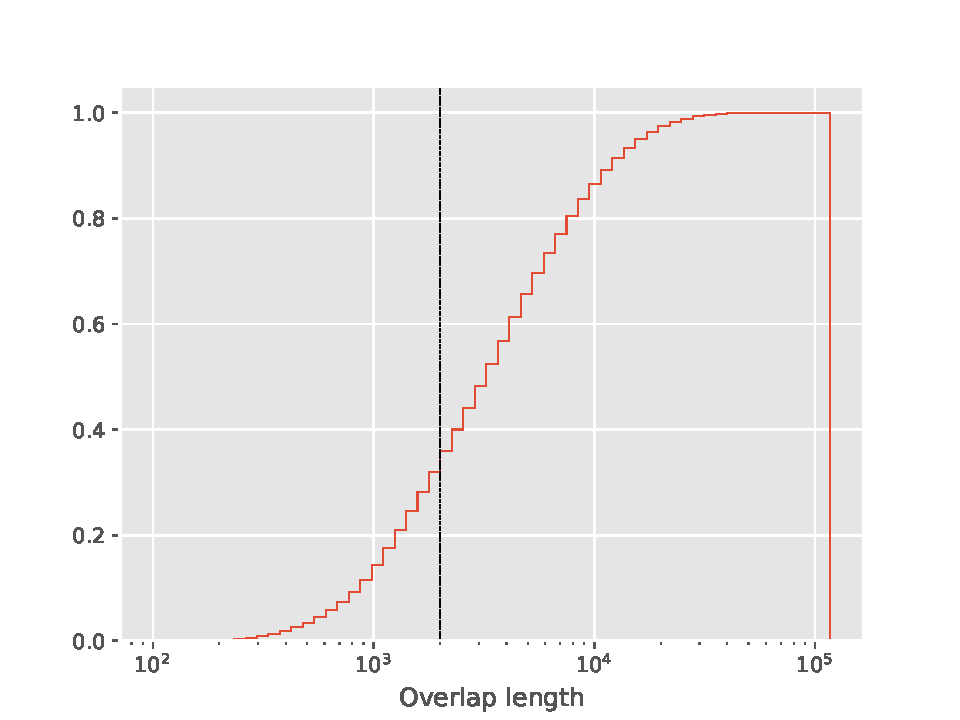
\includegraphics[width=\textwidth]{introduction/images/overlap_length.pdf}
    \caption{Histogram of overlap length found by \minimap, the black line represent the \miniasm length threshold. The fasta file weight 3.1 Go, complete PAF file generate by \minimap weight 5.5 Go, without overlap lower than 2000 bases weight was 3.7 Go.}
    \label{intro:fig:length_overlap_histogram}
\end{figure}

Can we filter overlapping information with a positive (or not very bad) impact on assembly result, to increase speed of assembly and the impact of assembly step on disk space ?

We present our solution of this problem \fpa (for Filter Pairwise Alignment) in section \ref{section:preassembly:paper}, overlaper output can by pipe directly in \fpa , \fpa can filter overlap with some filter, length of read, length of overlap, type of overlap, read name. Some simple \fpa filter reduce the computation time of assembly without effect (or a small positive effect) on assembly, read section \ref{section:preassembly:paper} for more details on this tools.


\section{Read scrubbing an alternative of read correction} \label{sec:preasm:intro_yacrd}

Assembly tools are based on reads. If your reads are bad, your assembly will be bad. To continue on the analogy given in the introduction, you probably cannot reconstruct a book if crazy monks gave to you only fragments with half of the letters being erroneous. Correction of reads, with a mix of sequencing technologies (or with a single technology), can help you to get better reads. But actually, correction tools have an important cost in term of computation time and memory usage. Moreover it's hard to differentiate natural mutations (e.g. real SNPs) to sequencing errors, and sometimes interesting mutations are consider as errors and are corrected (thus removed).

Correction was per-processing step to found and remove error in reads, this step was particularly important for long-reads data because her error rate was important and can lead to more error and misassembly in assembly. Roughly correction use overlap information to pick other reads share same sequence of a read need to be correct and use all information present sequence to build a consensus, we can cite tools like \toolsname{Mecat}\cite{MECAT}, \toolsname{CONSENT}\cite{CONSENT}. A similar task call polishing, was run after assembly, read are mapped against contig and contig sequence was correct with reads information we can site \toolsname{Racon}\cite{racon} and \toolsname{CONSENT}.

More than read contains error more correction required many reads, but the sequencing depth is not homogeneous and if for a given region this depth is not sufficient for the corrector, it will be less effective but it could still reduce the sequencing depth by eliminating reads or part of reads. To solve this problem it is necessary either to work without correction or to return to the raw reads to find the lost connection.

At the best of our knowledge the only one reads correctors they try to keept the hetrozygotie during correction is falcon \cite{falcon}, the other didn't try to keep this information. Or heterozygotie are very use full to understand genetic diversity in population or some genetic disease.
Moreover if you genome contain some almost repetion (two instance of same text with some mutation), the correction maybe can't distinguish the mutation between this two instance to sequencing error and correct the two instance of the almost repetition to the same sequence, so correction can create a repetition that cannot be resolved where there were we have two solvable almost repetitions.

Correction of reads before assembly can generate some trouble in assembly by remove some important read. But long-reads still contains very low quality region \cite{blog_post_error_repartition} this region can lead to a fragmented assembly \cite{long_read_assembler_comparison}. An alternative to preassembly correction can be scrubbing, remove only very low quality region and keep all other information.

To found and remove this very low quality region and read we create \yacrd (for Yet Another Chimeric Read Detector), \yacrd use self overlapping information to compute a coverage curve and identify region with low coverage. We suppose this low coverage region is region with low quality, read section \ref{section:preassembly:paper} for more details on this tools.


Our paper "\yacrd and \fpa: upstream tools for long-read genome assembly" presents two tools, \yacrd , and \fpa. \yacrd focuses on the detection and elimination of very poor quality regions. \fpa focuses on filtering 'useless' overlaps.



\subfile{paper/yacrd_fpa.tex}

\section{Chapter conclusion}

The blog post on overlapping tools comparaison, demonstrate overlapping tools didn't found same overlap. And that we will be able to improve the quality of the overlaps we found between our reads by combining their results. This is the idea of an overlaps consensus generator. But in the blog post we consider if two overlapping tools found a overlap between same reads they found the same overlap. But in a case of two reads \texttt{A} and \texttt{B}, it's possible:
\begin{itemize}
    \item the first overlapping tools found the end of read \texttt{A} overlap the begin of read \texttt{B}
    \item the second overlapping tools found the end of read \texttt{B} overlap the begin of read \texttt{A}
    \item the third overlapping tools found the reads \texttt{A} and \texttt{B} share an internal match
\end{itemize}

This list can be continued indefinitely. If we want build a overlaps consensus generator we need found a method, to say this two overlap found by two different overlapping tools, concern the same region of read \texttt{A} and the same region of read \texttt{B}, we can increase our confidence in this overlap is a \textit{true} overlap and it's is between this region of \texttt{A} and this region of read \texttt{B}. Or all overlapping tools found an overlap between read \texttt{C} and \texttt{D} but all this overlap concern different region of \texttt{C} and \texttt{D}, we can say they are probably no overlap between \texttt{C} and \texttt{D}.
This work was made in the context of a PFE (\textit{Projet de Fin d'Étude} End of Study Projects) by Yann Grabe. He create a tool that will build a consensus of several overlap files, by founding overlap between overlap and compute a confident score on each overlap by evaluate the number of overllaping tools found the same overlap.

For the moment this tool is only a prototype and would still require a lot of work before it can be finalized. 

\yacrd and \fpa have an important impact on assembly of \miniasm and \wtdbg. They were well received by the community \yacrd and \fpa was actually used, in some tools and pipeline.

\pim{Trouvé une conclusion globale au chapitre}

%\onlyinsubfile{
%\bibliographystyle{plainnat}
%\bibliography{main}
%\addcontentsline{toc}{chapter}{Bibliography}
%}

\end{document}